% Specifica Tecnica
% da compilare con il comando pdflatex Specifica_tecnica_x.x.x.tex

% Dichiarazioni di ambiente e inclusione di pacchetti
% da usare tramite il comando % Dichiarazioni di ambiente e inclusione di pacchetti
% da usare tramite il comando % Dichiarazioni di ambiente e inclusione di pacchetti
% da usare tramite il comando \input{../../util/hx-ambiente}

\documentclass[a4paper,titlepage]{article}
\usepackage[T1]{fontenc}
\usepackage[utf8]{inputenc}
\usepackage[english,italian]{babel}
\usepackage{microtype}
\usepackage{lmodern}
\usepackage{underscore}
\usepackage{graphicx}
\usepackage{eurosym}
\usepackage{float}
\usepackage{fancyhdr}
\usepackage[table]{xcolor}
\usepackage{longtable}
\usepackage{chngpage}
\usepackage{grffile}
\usepackage[titles]{tocloft}
\usepackage{hyperref}
\hypersetup{hidelinks}

\usepackage{../../util/hx-vers}
\usepackage{../../util/hx-macro}
\usepackage{../../util/hx-front}

% solo se si vuole una nuova pagina ad ogni \section:
\usepackage{titlesec}
\newcommand{\sectionbreak}{\clearpage}

% stile di pagina:
\pagestyle{fancy}

% solo se si vuole eliminare l'indentazione ad ogni paragrafo:
\setlength{\parindent}{0pt}

% intestazione:
\lhead{\Large{\proj}}
\rhead{
\includegraphics[keepaspectratio=true,width=50px]{../../util/hivex_logo2.png}}
\renewcommand{\headrulewidth}{0.4pt}

% pie' di pagina:
\lfoot{\email}
\rfoot{\thepage}
\cfoot{}
\renewcommand{\footrulewidth}{0.4pt}

% spazio verticale tra le celle di una tabella:
\renewcommand{\arraystretch}{1.5}

% profondità di indicizzazione:
\setcounter{tocdepth}{4}
\setcounter{secnumdepth}{4}


\documentclass[a4paper,titlepage]{article}
\usepackage[T1]{fontenc}
\usepackage[utf8]{inputenc}
\usepackage[english,italian]{babel}
\usepackage{microtype}
\usepackage{lmodern}
\usepackage{underscore}
\usepackage{graphicx}
\usepackage{eurosym}
\usepackage{float}
\usepackage{fancyhdr}
\usepackage[table]{xcolor}
\usepackage{longtable}
\usepackage{chngpage}
\usepackage{grffile}
\usepackage[titles]{tocloft}
\usepackage{hyperref}
\hypersetup{hidelinks}

\usepackage{../../util/hx-vers}
\usepackage{../../util/hx-macro}
\usepackage{../../util/hx-front}

% solo se si vuole una nuova pagina ad ogni \section:
\usepackage{titlesec}
\newcommand{\sectionbreak}{\clearpage}

% stile di pagina:
\pagestyle{fancy}

% solo se si vuole eliminare l'indentazione ad ogni paragrafo:
\setlength{\parindent}{0pt}

% intestazione:
\lhead{\Large{\proj}}
\rhead{
\includegraphics[keepaspectratio=true,width=50px]{../../util/hivex_logo2.png}}
\renewcommand{\headrulewidth}{0.4pt}

% pie' di pagina:
\lfoot{\email}
\rfoot{\thepage}
\cfoot{}
\renewcommand{\footrulewidth}{0.4pt}

% spazio verticale tra le celle di una tabella:
\renewcommand{\arraystretch}{1.5}

% profondità di indicizzazione:
\setcounter{tocdepth}{4}
\setcounter{secnumdepth}{4}


\documentclass[a4paper,titlepage]{article}
\usepackage[T1]{fontenc}
\usepackage[utf8]{inputenc}
\usepackage[english,italian]{babel}
\usepackage{microtype}
\usepackage{lmodern}
\usepackage{underscore}
\usepackage{graphicx}
\usepackage{eurosym}
\usepackage{float}
\usepackage{fancyhdr}
\usepackage[table]{xcolor}
\usepackage{longtable}
\usepackage{chngpage}
\usepackage{grffile}
\usepackage[titles]{tocloft}
\usepackage{hyperref}
\hypersetup{hidelinks}

\usepackage{../../util/hx-vers}
\usepackage{../../util/hx-macro}
\usepackage{../../util/hx-front}

% solo se si vuole una nuova pagina ad ogni \section:
\usepackage{titlesec}
\newcommand{\sectionbreak}{\clearpage}

% stile di pagina:
\pagestyle{fancy}

% solo se si vuole eliminare l'indentazione ad ogni paragrafo:
\setlength{\parindent}{0pt}

% intestazione:
\lhead{\Large{\proj}}
\rhead{
\includegraphics[keepaspectratio=true,width=50px]{../../util/hivex_logo2.png}}
\renewcommand{\headrulewidth}{0.4pt}

% pie' di pagina:
\lfoot{\email}
\rfoot{\thepage}
\cfoot{}
\renewcommand{\footrulewidth}{0.4pt}

% spazio verticale tra le celle di una tabella:
\renewcommand{\arraystretch}{1.5}

% profondità di indicizzazione:
\setcounter{tocdepth}{4}
\setcounter{secnumdepth}{4}


\version{0.0.1}
\creaz{15 febbraio 2017}
\author{...}
\supervisor{...}
\uso{esterno}
\dest{\ALL}
\title{Specifica Tecnica}
% \date{9 gennaio 2017}

\begin{document}
\maketitle
% diario delle modifiche per il piano di progetto
% da includere con % diario delle modifiche per il piano di progetto
% da includere con % diario delle modifiche per il piano di progetto
% da includere con \include{diario}

\begin{diario}
	1.0.1 & {\GG} (Responsabile) & 03/02/2017 & Correzione degli errori individuati nelle prime tre sezioni del documento \\ \hline
	1.0.0 & {\PB} (Responsabile) & 09/01/2017 & Approvazione documento \\ \hline
	0.1.0 & {\MM} (Verificatore) & 07/01/2017 & Verifica documento \\ \hline
	0.0.9 & {\PB} (Responsabile) & 05/01/2017 & Stesura Organigramma \\ \hline
	0.0.8 & {\LB} (Responsabile) & 05/01/2017 & Stesura Consuntivo di Periodo \\ \hline
	0.0.7 & {\LB} (Responsabile) & 04/01/2017 & Stesura Preventivo di Periodo \\ \hline
	0.0.6 & {\LB} (Responsabile) & 03/01/2017 & Inserimento Gantt Diagrammi delle Attività \\ \hline
	0.0.5 & {\PB} (Responsabile) & 29/12/2016 & Stesura Pianificazione delle Attività \\ \hline
	0.0.4 & {\PB} (Responsabile) & 28/12/2016 & Stesura Introduzione \\ \hline
	0.0.3 & {\LB} (Responsabile) & 27/12/2016 & Stesura Modello di sviluppo \\ \hline
	0.0.2 & {\PB} (Responsabile) & 27/12/2016 & Stesura Analisi dei Rischi \\ \hline
	0.0.1 & {\LB} (Responsabile) & 26/12/2016 & Stesura scheletro \\ \hline
\end{diario}

\begin{diario}
	1.0.1 & {\GG} (Responsabile) & 03/02/2017 & Correzione degli errori individuati nelle prime tre sezioni del documento \\ \hline
	1.0.0 & {\PB} (Responsabile) & 09/01/2017 & Approvazione documento \\ \hline
	0.1.0 & {\MM} (Verificatore) & 07/01/2017 & Verifica documento \\ \hline
	0.0.9 & {\PB} (Responsabile) & 05/01/2017 & Stesura Organigramma \\ \hline
	0.0.8 & {\LB} (Responsabile) & 05/01/2017 & Stesura Consuntivo di Periodo \\ \hline
	0.0.7 & {\LB} (Responsabile) & 04/01/2017 & Stesura Preventivo di Periodo \\ \hline
	0.0.6 & {\LB} (Responsabile) & 03/01/2017 & Inserimento Gantt Diagrammi delle Attività \\ \hline
	0.0.5 & {\PB} (Responsabile) & 29/12/2016 & Stesura Pianificazione delle Attività \\ \hline
	0.0.4 & {\PB} (Responsabile) & 28/12/2016 & Stesura Introduzione \\ \hline
	0.0.3 & {\LB} (Responsabile) & 27/12/2016 & Stesura Modello di sviluppo \\ \hline
	0.0.2 & {\PB} (Responsabile) & 27/12/2016 & Stesura Analisi dei Rischi \\ \hline
	0.0.1 & {\LB} (Responsabile) & 26/12/2016 & Stesura scheletro \\ \hline
\end{diario}

\begin{diario}
	1.0.1 & {\GG} (Responsabile) & 03/02/2017 & Correzione degli errori individuati nelle prime tre sezioni del documento \\ \hline
	1.0.0 & {\PB} (Responsabile) & 09/01/2017 & Approvazione documento \\ \hline
	0.1.0 & {\MM} (Verificatore) & 07/01/2017 & Verifica documento \\ \hline
	0.0.9 & {\PB} (Responsabile) & 05/01/2017 & Stesura Organigramma \\ \hline
	0.0.8 & {\LB} (Responsabile) & 05/01/2017 & Stesura Consuntivo di Periodo \\ \hline
	0.0.7 & {\LB} (Responsabile) & 04/01/2017 & Stesura Preventivo di Periodo \\ \hline
	0.0.6 & {\LB} (Responsabile) & 03/01/2017 & Inserimento Gantt Diagrammi delle Attività \\ \hline
	0.0.5 & {\PB} (Responsabile) & 29/12/2016 & Stesura Pianificazione delle Attività \\ \hline
	0.0.4 & {\PB} (Responsabile) & 28/12/2016 & Stesura Introduzione \\ \hline
	0.0.3 & {\LB} (Responsabile) & 27/12/2016 & Stesura Modello di sviluppo \\ \hline
	0.0.2 & {\PB} (Responsabile) & 27/12/2016 & Stesura Analisi dei Rischi \\ \hline
	0.0.1 & {\LB} (Responsabile) & 26/12/2016 & Stesura scheletro \\ \hline
\end{diario}
\tableofcontents
\listofpattern



% - introduzione standard
% - stime di fattibilità
\section{Introduzione}
%%%%%%%%%%%%%%%%
%%  Introduzione
%%%%%%%%%%%%%%%%

\subsection{Scopo del documento}
Questo documento ha lo scopo di definire, ad alto livello, l'architettura software di \proj; ci focalizziamo quindi sulla \emph{struttura} del software, cioè sulla descrizione delle sue componenti. L'implementazione del nostro software è a oggetti; per questo, le componenti descritte sono classi e loro istanze.
% Ecco una prova di pattern: \pattern{Observer}

Riteniamo che l'architettura esposta di seguito, accompagnata da un documento più preciso che verrà prodotto nelle prossime settimane (Definizione di Prodotto), sia ragionevole e fattibile. La difficoltà di generare codice eseguibile è stata superata grazie ad un uso accorto di librerie open-source, stili architetturali e \emph{design patter}. Il tutto è stato svolto con grande attenzione ai princìpi della programmazione ad oggetti, per aumentare il grado di coesione di un'architettura che rischia ad ogni momento di gonfiarsi inutilmente.

Ci è parso utile indicizzare i \emph{design patter} utilizzati; per questo, li abbiamo riportati in un elenco (dopo l'indice generale).

\subsection{Scopo del prodotto}
\scopo

\subsection{Glossario}
\presgloss

\subsection{Riferimenti} \label{sec:ref}

\subsubsection{Riferimenti normativi}
% ...

\subsubsection{Riferimenti informativi}
\begin{itemize}
	\item E. Gamma, R. Helm, R. Johnson, J. Vlissides, \emph{Design Patterns: Elements of Reusable Object-Oriented Software}.
\end{itemize}


% - scelta di linguaggi, framework, librerie etc...
% - interfacce con tali tecnologie
\section{Tecnologie utilizzate}
%%%%%%%%%%%%%%%%%%%%%%%%%
%%  Tecnologie utilizzate
%%%%%%%%%%%%%%%%%%%%%%%%%



\subsection{\gloss{Client}}
Per implementare il client di \proj{} abbiamo scelto di utilizzare \gloss{HTML5} e \gloss{CSS3} assieme a \gloss{JavaScript}. Di seguito elenchiamo e descriviamo le librerie JavaScript di cui il nostro client necessita. Tutte le librerie sono open-source, come richiesto dal capitolato.

\subsubsection{JointJS}
La libreria \jointjs{} (\url{https://www.jointjs.com/opensource}) è una libreria open-source per realizzare \gloss{editor} di diagrammi interattivi, in maniera altamente personalizzabile. %Dipende da HTML5 e da alcune altre librerie JavaScript ma offre numerosi plug-in per realizzare particolari tipi di grafi.

La libreria sfrutta le seguenti tecnologie per il suo funzionamento:

\begin{itemize}
	\item \\gloss{html}{}: \jointjs{} richiede che una pagina \html{} sia popolata con un tag \texttt{<svg>}, che conterrà un diagramma.
	\item Le seguenti librerie \js{}:
	\begin{itemize}
		\item \jquery{};
		\item \lodash{};
		\item \backbonejs{}.
	\end{itemize}
\end{itemize}

\subsubsection{\backbonejs}
La libreria \backbonejs{} permette di strutturare applicazioni web single page (SPA) fornendo \textbf{modelli} con binding di chiave-valore, eventi, \textbf{collezioni} e \textbf{viste} con una gestione degli eventi dichiarativa. Essa offre inoltre una interfaccia RESTful.

A causa della struttura data alla libreria \jointjs{}, sviluppata tramite MVC (collection), al fine di ridurre il numero di librerie necessarie allo sviluppo del progetto, si costruirà \proj{} estendendo le funzionalità di base offerte da \jointjs{} usando il modello \mvc{}.


\subsubsection{\jquery}
La libreria \jquery{} è sfruttata da \jointjs{} ed è necesaria per semplificare varie operazioni di basso livello. 


\subsubsection{\requirejs}
La libreria \requirejs{} è un loader di moduli e file \js{}. Esso si occuperà principalmente di risolvere dipendenze delle librerie \js{} utilizzate.

\subsubsection{\lodash}
La libreria \lodash{} fornisce metodi di utilità non offerti da \js{} puro. Rispetto alla simile libreria \emph{Underscore}, questa fornisce più performance, più features e miglior documentazione. Essa inoltre è usata da \jointjs{}.

\subsection{\gloss{Server}}

\subsubsection{Apache \gloss{Tomcat}}
% ...

\subsubsection{Pivotal Spring}
% ...

%%% [altro...]



\subsection{Linguaggio target}

%%% [...]


% - diagramma dei package
% - scelte architetturali
% - altre cose ad alto livello
\section{Descrizione dell'architettura}
%%%%%%%%%%%%%%%%%%%%%%%%%%%%%%%%%
%%  Descrizione dell'architettura
%%%%%%%%%%%%%%%%%%%%%%%%%%%%%%%%%



\subsection{Metodo e formalismo di specifica}
La descrizione dell'architettura di \proj{} è suddivisa in quattro sezioni:
\begin{itemize}
	\item §\ref{sec:arch_gen}, che illustra gli aspetti generali dell'architettura del software;
	\item §\ref{sec:arch_client}, che descrive l'architettura del \emph{front end} dell'applicazione;
	\item §\ref{sec:arch_server}, che descrive l'architettura del \emph{back end} dell'applicazione;
	\item §\ref{sec:arch_proto}, che descrive il protocollo che lega le due interfacce precedenti.
\end{itemize}
Per ognuna di queste sezioni, procediamo con metodo \emph{top-down} --- dal generale al particolare. utilizziamo dei diagrammi che seguono i formalismi di UML 2.0 e in essi, evidenziamo in colore più scuro le parti dell'architettura che sono di librerie esterne.



\subsection{Descrizione generale} \label{sec:arch_gen}
L'architettura dell'applicazione è suddivisa in due moduli:
\begin{enumerate}
	\item il client, che vive nel browser dell'utente;
	\item il server, che fornisce la pagina dell'applicazione al client e riceve da esso delle richieste di generazione di codice.
\end{enumerate}

Tra le varie qualità desiderabili per la nostra architettura, la progettazione ha perseguito principalmente l'\textbf{estensibilità}. Tale obiettivo è stato raggiunto con due strategie:
\begin{itemize}
	\item in generale, promuovendo le seguenti qualità:
	\begin{itemize}
		\item manutenibilità;
		\item modularità;
		\item semplicità;
		\item basso accoppiamento.
	\end{itemize}
	\item nello specifico, prevedendo le seguenti possibili aggiunte nel futuro:
	\begin{itemize}
		\item Generazione di codice in altri linguaggi target: se i manutentori vorranno generare del codice JavaScript o Python, sarà sufficiente aggiungere dei template per il linguaggio scelto (grazie alla libreria \emph{StringTemplate}).
		\item Diversa compressione del codice generato: attualmente l'applicazione genera un JAR e lo comprime, assieme al file JSON, in formato ZIP; ma si potrebbe facilmente cambiare il formato di compressione in un JAR che contenga egli stesso al suo interno il file JSON.
		\item Persistenza dei dati del diagramma che arrivano in input al \emph{back end}: si potrebbe voler mantenere un database di utenti dell'applicazione, ognuno con i propri diagrammi mantenuti nel server a tempo indefinito; per questo, basta fornire l'indirizzo della risorsa JSON, che attualmente non viene eliminata dal server. % (oppure per ora potremmo eliminarla...)
		\item Persistenza del programma generato: si potrebbe voler mantenere anche il codice generato, come il diagramma di input; per fare ciò, basta garantire al client il carattere persistente della risorsa fornita (badando però a non eliminarla dal server). % (per ora la eliminiamo?)
		\item Diverso formato per i diagrammi in input: si potrebbe voler ricevere dei dati da un client esterno, anziché in JSON (e.g. disegnatori di diagrammi UML come Astah); sarà sufficiente modificare il package \texttt{parser}.
		\item Aumento del numero di stereotipi UML offerti: la presenza di un numero consistente di stereotipi non sarà mai un problema, grazie al fatto che vengono caricati dinamicamente nel client in modo asincrono.
	\end{itemize}
\end{itemize}



\subsection{Architettura del client} \label{sec:arch_client}
Il \emph{front end} di \proj{} è una \emph{Single Page Application} (\gloss{SPA}) scritta in HTML5, CSS3 e JavaScript.

L'\texttt{head} (intestazione) della pagina HTML contiene dei puntatori a:
\begin{itemize}
	\item le librerie JavaScript elencate nella sezione \ref{sec:tech_client} (con eventuali relativi fogli CSS);
	\item il foglio di stile CSS della pagina;
	\item lo script JavaScript che utilizza le librerie di cui sopra.
\end{itemize}

Il \texttt{body} (corpo) della pagina HTML si compone di pochi blocchi:
\begin{itemize}
	\item dei tag \texttt{div} contenenti i menù laterali da cui selezionare gli strumenti e gli elementi per interagire con i diagrammi;
	\item un tag \texttt{svg} (identificato dall'\texttt{id} \emph{paper}) che contiene, di volta in volta, il diagramma delle classi o il diagramma di un metodo particolare.
\end{itemize}
Alla ricezione della pagina da parte del client, lo script JavaScript popola il tag \texttt{svg} (inizialmente vuoto) con un diagramma delle classi vuoto.

L'architettura del client è suddivisa in tre moduli, come in figura \ref{fig:client_pkg}:
\begin{itemize}
	\item \texttt{model}, che organizza la logica sottostante i diagrammi;
	\item \texttt{view}, che gestisce l'interfaccia grafica;
	\item \texttt{collection}, che raggruppa in una collezione più model, come per tutti i diagrammi creati. % <<< ?
\end{itemize}

\texttt{model} contiene i vari tipi di celle dei diagrammi: elementi del diagramma delle classi, collegamenti tra essi, stereotipi per giochi da tavolo e, infine, elementi dei diagrammi a blocchi. % ...

\texttt{view} offre la classe \texttt{ProjectView}, che rappresenta l'area di disegno principale dell'applicazione. Attorno ad essa sono presenti dei menù: \texttt{DetailsView} visualizza tutti i campi di un elemento o di un collegamento tra elementi e ne permette la modifica; \texttt{NewCellView} visualizza tutti i possibili tipi di elementi e collegamenti che si possono inserire in un diagramma. Tutta l'interfaccia grafica è orchestrata da una \texttt{AppView}, che crea una \texttt{ProjectView}, una \texttt{DetailsView} e una \texttt{NewCellView}.

\texttt{collection} contiene soltanto la classe \texttt{DiagramCollection}, che compone in una collezione più oggetti \texttt{Cell} (tipo definito da \jointjs). Ognuno di questi oggetti è l'elemento di un diagramma (a classi o a blocchi) oppure un collegamento tra elementi del diagramma delle classi.

% diagramma dei package del client
\begin{figure} \label{fig:client_pkg}
	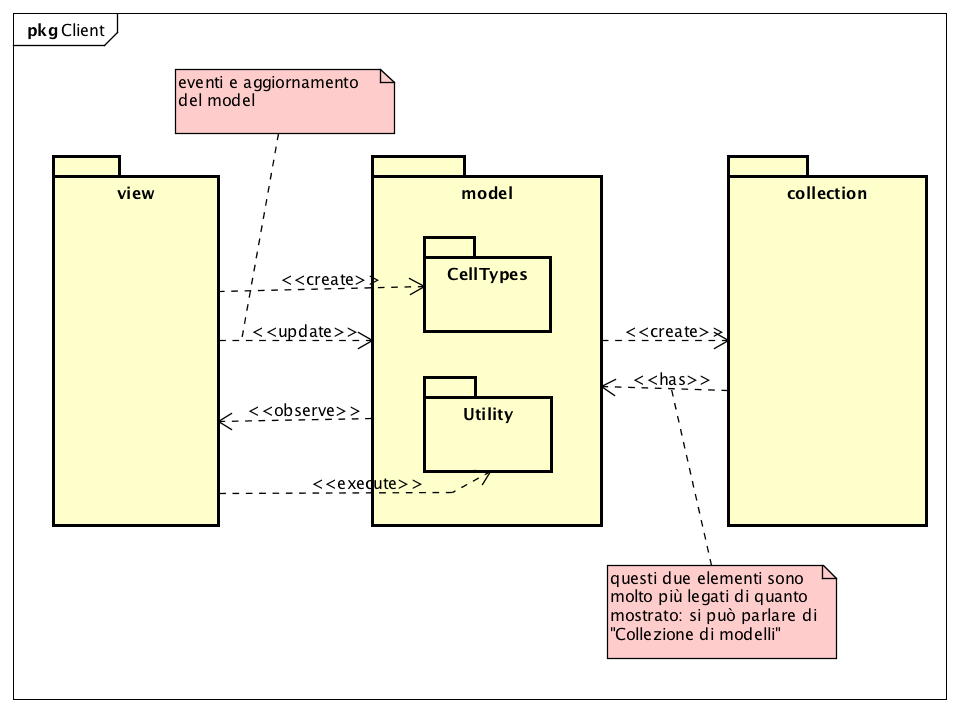
\includegraphics[scale=0.5]{img/client_pkg}
	\caption{Architettura del client.}
\end{figure}



\subsection{Architettura del server} \label{sec:arch_server}
Il server offre tre servizi:
\begin{enumerate}
	\item fornisce al client la pagina HTML dove disegnare i diagrammi;
	\item restituisce l'elenco degli stereotipi esistenti all'interno del server e utilizzabili dal client;
	\item elabora un file JSON in arrivo dal client e gli fornisce l'applicazione generata a partire da tale file.
\end{enumerate}
Questi tre servizi rispettano lo stile architetturale REST (come spiegato più avanti nella sezione \ref{sec:arch_proto}).

Il primo servizio è una semplice pagina HTML, fornita normalmente da Tomcat e arricchita di codice Javascript.

Il secondo e il terzo servizio, invece, sono un programma Java che genera due \emph{servlet}; il programma è organizzato nei seguenti package, come illustrato in figura \ref{fig:server_pkg}:
\begin{itemize}
	\item \textbf{\texttt{controller}} rappresenta il nucleo del \emph{back end}; un \texttt{RequestHandlerController} si occupa di generare le due \emph{servlet} Java, usando \emph{Spring}.
	\item nel package \textbf{\texttt{parser}}, la classe \texttt{Parser} si occupa di convertire il file JSON ricevuto in un oggetto Java di tipo \texttt{ParsedProgram}. Questo oggetto Java rappresenta il programma che l'utente vuole generare; esso si compone di oggetti \texttt{ParsedType} (cioè i tipi definiti dall'utente: gli elementi del diagramma delle classi), i quali si possono comporre di oggetti \texttt{ParsedAttribute} e \texttt{ParsedMethod}; quest'ultimo tipo si compone a sua volta di oggetti \texttt{ParsedInstruction} e così via fino ad arrivare alle istruzioni “atomiche”, come per esempio un \texttt{ParsedReturn}.
	\item \textbf{\texttt{project}} non è altro che il package che organizza i tipi elencati al punto precedente, tutti discendenti da \texttt{ParsedElement}. Inoltre, questo package offre una classe \texttt{ElementFactory}. % che non ho capito cosa fa
	\item \textbf{\texttt{generator}} presenta al suo interno l'interfaccia \texttt{Generator}; le classi che la estendono si occupano di popolare i template \emph{StringTemplate} di un particolare linguaggio di programmazione (\texttt{JavaGenerator} genera codice sorgente Java) e scrivere il risultato su disco. \texttt{GeneratorAssembler} fornisce la giusta implementazione \texttt{Generator}, grazie a un file di configurazione XML e a \emph{Spring}.
	\item \textbf{\texttt{template}} è il package che organizza i template per linguaggio: dall'interfaccia \texttt{Template} discende, ad esempio, \texttt{JavaTemplate}. Anche questo package presenta una classe che si occupa di fornire la giusta implementazione di \texttt{Template}: \texttt{TemplateAssembler}, dipendente anch'esso dal file di configurazione XML.
	\item \textbf{\texttt{stereotype}} espone una classe che recupera da disco i vari template di ogni stereotipo implementato.
	\item \textbf{\texttt{compiler}} presenta l'interfaccia \texttt{Compiler}, le cui implementazioni specifiche (per un certo linguaggio target) compilano il codice sorgente non eseguibile in un programma eseguibile (che viene poi scritto su disco); \texttt{JavaCompiler}, ad esempio, compila codice sorgente Java in \emph{bytecode} per la JVM (Java Virtual Machine) e compatta il codice in un file JAR eseguibile. Anche questo package presenta un \texttt{CompilerAssembler} (dipendente dal file di configurazione XML) che si occupa di fornire la giusta implementazione di \texttt{Compiler}.
	\item \textbf{\texttt{utility}} espone classi di utilità per il programma, come ad esempio una classe \texttt{Compressor} che comprime l'output di un \texttt{Compiler} in formato ZIP. % è pulito tenere un package con un nome così generico?
\end{itemize}

% >>> diagr. dei package del server
\begin{figure} \label{fig:server_pkg}
	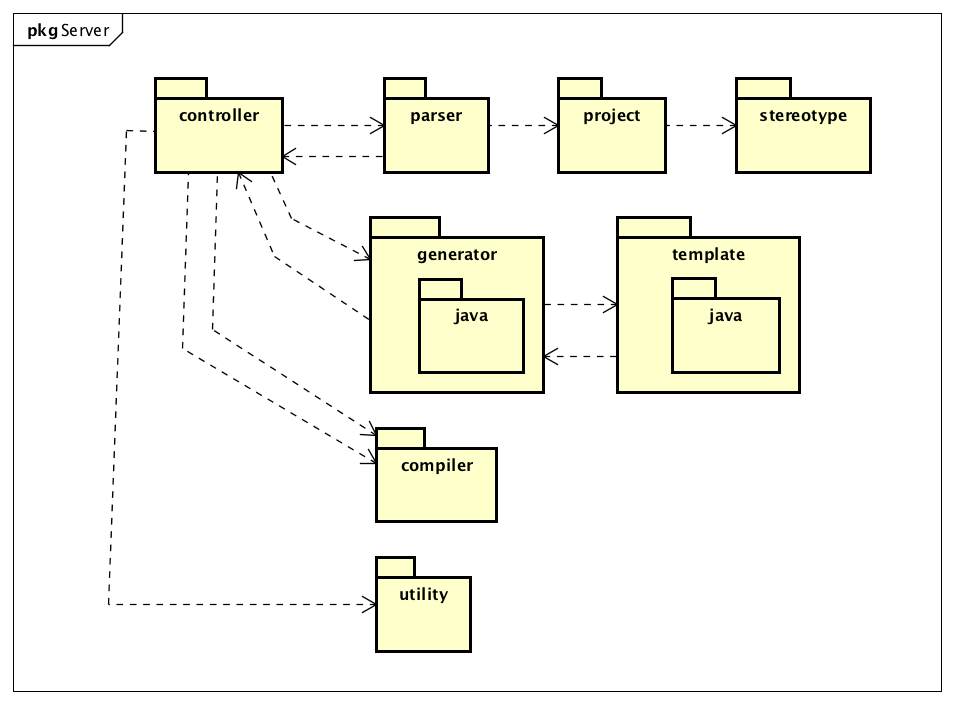
\includegraphics[scale=0.5]{img/server_pkg}
	\caption{Architettura del server.}
\end{figure}



\subsection{Protocollo di comunicazione client-server} \label{sec:arch_proto}
I tre servizi offerti dal server (ottenere la pagina HTML; recuperare stereotipi UML; ottenere l'applicazione generata) seguono lo stile architetturale REST:
\begin{itemize}
	\item La richiesta per ottenere la pagina HTML usa il metodo HTTP GET; la pagina è quindi \emph{cachable} (i router tra client e server possono decidere di ottimizzarne la fornitura).
	\item Il file JSON viene spedito con il metodo HTTP POST, che permette la persistenza di tale file nel server; la persistenza del file JSON è indifferente alla nostra applicazione ma ne aumenta l'estensibilità, in quanto un giorno i manutentori potrebbe voler offrire un servizio di condivisione dei diagrammi disegnati oppure un database di utenti che abbiano i propri diagrammi sul server.
	\item Ognuno dei tre servizi (pagina HTML, recupero di stereotipi e generazione di codice) è una risorsa distinta: questo disaccoppia i due servizi, aumentando ancora la manutenibilità del sistema.
	\item La richiesta per ottenere la pagina HTML è per forza idempotente: lo stato del server non può influire su una pagina statica. %Neanche il recupero di stereotipi dipende dallo stato del server, dato che gli stereotipi sono contenuti in file statici. % <<< o forse no?
	\item La richiesta di generazione di codice è idempotente: l'unica dipendenza esterna al programma è il file JSON, che viene passato dal client.
\end{itemize}

\begin{figure} \label{fig:protocol}
	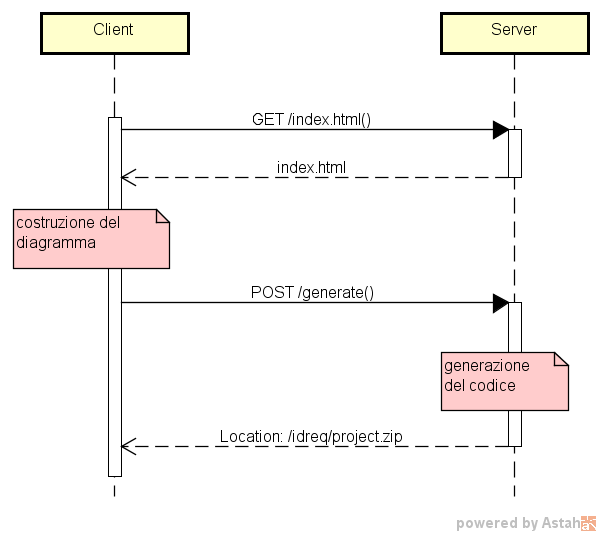
\includegraphics[scale=0.66]{img/http}
	\caption{Possibile interazione tra client e server.}
\end{figure}

% ci sarebbe da fare pure una cosa simile per il recupero degli stereotipi


% ---> distinguere STRUTTURA (classi) da COMPORTAMENTO (procedure)?
% - diagrammi delle classi
% - se serve, qualche diagramma di attività/sequenza
\section{Componenti}
%%%%%%%%%%%%%%
%%  Componenti
%%%%%%%%%%%%%%



% [Breve introduzione...]



\subsection{Client}

\subsubsection{MainApp}
% ...

\subsubsection{AppView}
% ...

% eccetera...




\subsection{Server}
% server==package principale
%Controller== classe che fa da Front Controller
%generator== package dentro server che fa il lavoro di creare il zip
%Project==classe (forse interface o abstract) dentro generator che fa il lavoro di creare il zip
\subsubsection{server}
--immagine package server con la classe controller che comunica con la classe Project contenuta nel package generator--
\begin{description}
\item[Descrizione] è il package che racchiude tutte le componenti del back-end che si occupano di soddisfare le richieste provenienti dal front-end ed elaborarle;
\item[Package contenuti] 
	\begin{itemize}
	\item server::endpoints (in teoria non c'è);
	\item server::generator;
	\end{itemize}
\item[Interazione con altri componenti] interagisce con il client definito nella sez xxx tramite i servizi REST offerti. (in teoria non c'è)
\end{description}

\paragraph{Classi}
\subparagraph{server::Controller}
\begin{description}
\item[Descrizione] è la classe che implementa il pattern Front Controller e si occupa di raccogliere le richieste dal client (anche Singleton??)
\item[Utilizzo] viene invocata ""dal client"" e trasferisce la richiesta alla classe Project contenuta nel package server::generator che si occuperà di invocare il relativo comando per soddisfare la richiesta; 
\item[Relazioni con altre classi] 
	\begin{itemize}
	\item server::generator::Project.
	\end{itemize}
\end{description}

\subsubsection{server::generator}
--immagine--
\begin{description}
\item[Descrizione] è il package che contiene tutte le componenti che definiscono la logica necessaria per soddisfare le richieste il arrivo dal client;
\item[Padre] server; 
\item[Package contenuti]
	\begin{itemize}
	...
	\end{itemize}
\item[Interazione con altre componenti] 
	\begin{itemize}
	\item server::Controller.
	\end{itemize}
\end{description}


% JSON, client-server... ???
\section{Modelli dei dati e interfacce}
%%%%%%%%%%%%%%%%%%%%%%%%%%%%%%%%%
%%  Modelli dei dati e interfacce
%%%%%%%%%%%%%%%%%%%%%%%%%%%%%%%%%

%%% [...]


% - tracciamento componenti-reqq
% - tracciamento reqq-componenti
\section{Tracciamento}
%%%%%%%%%%%%%%%%
%%  Tracciamento
%%%%%%%%%%%%%%%%



In questa sezione tracciamo le corrispondenze tra componenti dell'architettura (classi) e requisiti, cioè:
\begin{enumerate}
	\item per ogni componente, i requisiti che ne motivano l'esistenza;
	\item per ogni requisito, le componenti che servono a soddisfarlo.
\end{enumerate}



\subsection{Tracciamento Classi-Requisiti}
\normalsize
\begin{longtable}{|>{\centering}m{10cm}|m{3cm}<{\centering}|}
\hline 
\textbf{Classe} & \textbf{Requisiti}\\
\hline
\endhead
\hyperref[\nogloxy{swedesigner::client::model::celltypes::activity::ActivityDiagramElement}]{\nogloxy{\texttt{swedesigner::client::model::celltypes::-\linebreak activity::ActivityDiagramElement}}} & RFO4\\ \hline

\hyperref[\nogloxy{swedesigner::client::model::celltypes::activity::HxCustom}]{\nogloxy{\texttt{swedesigner::client::model::celltypes::-\linebreak activity::HxCustom}}} & RFO4.6\\ \hline

\hyperref[\nogloxy{swedesigner::client::model::celltypes::activity::HxElse}]{\nogloxy{\texttt{swedesigner::client::model::celltypes::-\linebreak activity::HxElse}}} & RFO4.3\\ \hline

\hyperref[\nogloxy{swedesigner::client::model::celltypes::activity::HxFor}]{\nogloxy{\texttt{swedesigner::client::model::celltypes::-\linebreak activity::HxFor}}} & RFO4.5\\ \hline

\hyperref[\nogloxy{swedesigner::client::model::celltypes::activity::HxIf}]{\nogloxy{\texttt{swedesigner::client::model::celltypes::-\linebreak activity::HxIf}}} & RFO4.2\\ \hline

\hyperref[\nogloxy{swedesigner::client::model::celltypes::activity::HxReturn}]{\nogloxy{\texttt{swedesigner::client::model::celltypes::-\linebreak activity::HxReturn}}} & RFO4.33\\ \hline

\hyperref[\nogloxy{swedesigner::client::model::celltypes::activity::HxVariable}]{\nogloxy{\texttt{swedesigner::client::model::celltypes::-\linebreak activity::HxVariable}}} & RFO4.1\\ \hline

\hyperref[\nogloxy{swedesigner::client::model::celltypes::activity::HxWhile}]{\nogloxy{\texttt{swedesigner::client::model::celltypes::-\linebreak activity::HxWhile}}} & RFO4.4\\ \hline

\hyperref[\nogloxy{swedesigner::client::model::celltypes::class::ClassDiagramElement}]{\nogloxy{\texttt{swedesigner::client::model::celltypes::-\linebreak class::ClassDiagramElement}}} & RFO3\\
& RFD3.8\\
& RFD3.9\\ \hline

\hyperref[\nogloxy{swedesigner::client::model::celltypes::class::ClassDiagramLink}]{\nogloxy{\texttt{swedesigner::client::model::celltypes::-\linebreak class::ClassDiagramLink}}} & RFO3\\
& RFO3.4\\ \hline

\hyperref[\nogloxy{swedesigner::client::model::celltypes::class::HxAssociation}]{\nogloxy{\texttt{swedesigner::client::model::celltypes::-\linebreak class::HxAssociation}}} & RFO3.5\\
& RFO3.5.1\\
& RFO3.5.2\\ \hline

\hyperref[\nogloxy{swedesigner::client::model::celltypes::class::HxClass}]{\nogloxy{\texttt{swedesigner::client::model::celltypes::-\linebreak class::HxClass}}} & RFO3.1\\ \hline

\hyperref[\nogloxy{swedesigner::client::model::celltypes::class::HxComment}]{\nogloxy{\texttt{swedesigner::client::model::celltypes::-\linebreak class::HxComment}}} & RFD3.8\\ \hline

\hyperref[\nogloxy{swedesigner::client::model::celltypes::class::HxGeneralization}]{\nogloxy{\texttt{swedesigner::client::model::celltypes::-\linebreak class::HxGeneralization}}} & RFO3.6\\ \hline

\hyperref[\nogloxy{swedesigner::client::model::celltypes::class::HxImplementation}]{\nogloxy{\texttt{swedesigner::client::model::celltypes::-\linebreak class::HxImplementation}}} & RFD3.7\\ \hline

\hyperref[\nogloxy{swedesigner::client::model::celltypes::class::HxInterface}]{\nogloxy{\texttt{swedesigner::client::model::celltypes::-\linebreak class::HxInterface}}} & RFO3.3\\ \hline

\hyperref[\nogloxy{swedesigner::client::model::celltypes::HxStereotype}]{\nogloxy{\texttt{swedesigner::client::model::celltypes::-\linebreak HxStereotype}}} & RFO3.2.6\\ \hline

\hyperref[\nogloxy{swedesigner::client::model::NewCellFactory}]{\nogloxy{\texttt{swedesigner::client::model::-\linebreak NewCellFactory}}} & RFO3.1\\
& RFO3.3\\
& RFO4.1\\
& RFO4.2\\
& RFO4.3\\
& RFO4.4\\
& RFO4.5\\
& RFO4.6\\ \hline

\hyperref[\nogloxy{swedesigner::client::model::NewCellModel}]{\nogloxy{\texttt{swedesigner::client::model::-\linebreak NewCellModel}}} & RFO3.1\\
& RFO3.3\\
& RFO4.1\\
& RFO4.2\\
& RFO4.3\\
& RFO4.4\\
& RFO4.5\\
& RFO4.6\\ \hline

\hyperref[\nogloxy{swedesigner::client::model::ProjectCommand}]{\nogloxy{\texttt{swedesigner::client::model::-\linebreak ProjectCommand}}} & RFO2\\
& RFO5\\
& RFO6\\ \hline

\hyperref[\nogloxy{swedesigner::client::model::ProjectModel}]{\nogloxy{\texttt{swedesigner::client::model::-\linebreak ProjectModel}}} & RFO1.1\\
& RFO3\\
& RFO4\\ \hline

\hyperref[\nogloxy{swedesigner::client::model::utility::ProjectStereotypes}]{\nogloxy{\texttt{swedesigner::client::model::utility::-\linebreak ProjectStereotypes}}} & RFO3.2.6\\ \hline

\hyperref[\nogloxy{swedesigner::client::view::AppView}]{\nogloxy{\texttt{swedesigner::client::view::AppView}}} & RFO1\\
& RFO2\\
& RFO3\\
& RFO4\\
& RFO5\\
& RFO6\\ \hline

\hyperref[\nogloxy{swedesigner::client::view::DetailsView}]{\nogloxy{\texttt{swedesigner::client::view::DetailsView}}} & RFO3.12\\
& RFO3.13\\
& RFO3.14\\
& RFO3.15\\
& RFO3.18\\
& RFO4.27\\
& RFO4.28\\
& RFO4.29\\
& RFO4.30\\
& RFO4.31\\
& RFO4.32\\
& RFO4.34\\ \hline

\hyperref[\nogloxy{swedesigner::client::view::NewCellView}]{\nogloxy{\texttt{swedesigner::client::view::NewCellView}}} & RFO3.1\\
& RFO3.3\\
& RFO4.1\\
& RFO4.2\\
& RFO4.3\\
& RFO4.4\\
& RFO4.5\\
& RFO4.6\\ \hline

\hyperref[\nogloxy{swedesigner::client::view::ProjectView}]{\nogloxy{\texttt{swedesigner::client::view::ProjectView}}} & RFO3\\
& RFO4\\ \hline

\hyperref[\nogloxy{swedesigner::server::Application}]{\nogloxy{\texttt{swedesigner::server::Application}}} & RFO8\\ \hline

\hyperref[\nogloxy{swedesigner::server::compiler::Compiler}]{\nogloxy{\texttt{swedesigner::server::compiler::-\linebreak Compiler}}} & RFO9\\ \hline

\hyperref[\nogloxy{swedesigner::server::compiler::java::JavaCompiler}]{\nogloxy{\texttt{swedesigner::server::compiler::java::-\linebreak JavaCompiler}}} & RFO9\\ \hline

\hyperref[\nogloxy{swedesigner::server::controller::RequestHandlerController}]{\nogloxy{\texttt{swedesigner::server::controller::-\linebreak RequestHandlerController}}} & RFO7\\
& RFO8\\
& RFO9\\
& RFO10\\
& RFO11\\ \hline

\hyperref[\nogloxy{swedesigner::server::generator::Generator}]{\nogloxy{\texttt{swedesigner::server::generator::-\linebreak Generator}}} & RFO8.2\\ \hline

\hyperref[\nogloxy{swedesigner::server::generator::java::JavaGenerator}]{\nogloxy{\texttt{swedesigner::server::generator::java::-\linebreak JavaGenerator}}} & RFO8.2\\ \hline

\hyperref[\nogloxy{swedesigner::server::parser::Parser}]{\nogloxy{\texttt{swedesigner::server::parser::Parser}}} & RFO8.1\\ \hline

\hyperref[\nogloxy{swedesigner::server::project::ParsedAttribute}]{\nogloxy{\texttt{swedesigner::server::project::-\linebreak ParsedAttribute}}} & RFO8.1\\ \hline

\hyperref[\nogloxy{swedesigner::server::project::ParsedClass}]{\nogloxy{\texttt{swedesigner::server::project::-\linebreak ParsedClass}}} & RFO8.1\\ \hline

\hyperref[\nogloxy{swedesigner::server::project::ParsedCustom}]{\nogloxy{\texttt{swedesigner::server::project::-\linebreak ParsedCustom}}} & RFO8.1\\ \hline

\hyperref[\nogloxy{swedesigner::server::project::ParsedElement}]{\nogloxy{\texttt{swedesigner::server::project::-\linebreak ParsedElement}}} & RFO8.1\\ \hline

\hyperref[\nogloxy{swedesigner::server::project::ParsedElse}]{\nogloxy{\texttt{swedesigner::server::project::-\linebreak ParsedElse}}} & RFO8.1\\ \hline

\hyperref[\nogloxy{swedesigner::server::project::ParsedException}]{\nogloxy{\texttt{swedesigner::server::project::-\linebreak ParsedException}}} & RFO6.1\\ \hline

\hyperref[\nogloxy{swedesigner::server::project::ParsedFor}]{\nogloxy{\texttt{swedesigner::server::project::-\linebreak ParsedFor}}} & RFO8.1\\ \hline

\hyperref[\nogloxy{swedesigner::server::project::ParsedIf}]{\nogloxy{\texttt{swedesigner::server::project::ParsedIf}}} & RFO8.1\\ \hline

\hyperref[\nogloxy{swedesigner::server::project::ParsedInstruction}]{\nogloxy{\texttt{swedesigner::server::project::-\linebreak ParsedInstruction}}} & RFO8.1\\ \hline

\hyperref[\nogloxy{swedesigner::server::project::ParsedInterface}]{\nogloxy{\texttt{swedesigner::server::project::-\linebreak ParsedInterface}}} & RFO8.1\\ \hline

\hyperref[\nogloxy{swedesigner::server::project::ParsedMethod}]{\nogloxy{\texttt{swedesigner::server::project::-\linebreak ParsedMethod}}} & RFO8.1\\ \hline

\hyperref[\nogloxy{swedesigner::server::project::ParsedProgram}]{\nogloxy{\texttt{swedesigner::server::project::-\linebreak ParsedProgram}}} & RFO8.1\\ \hline

\hyperref[\nogloxy{swedesigner::server::project::ParsedReturn}]{\nogloxy{\texttt{swedesigner::server::project::-\linebreak ParsedReturn}}} & RFO8.1\\ \hline

\hyperref[\nogloxy{swedesigner::server::project::ParsedStatement}]{\nogloxy{\texttt{swedesigner::server::project::-\linebreak ParsedStatement}}} & RFO8.1\\ \hline

\hyperref[\nogloxy{swedesigner::server::project::ParsedType}]{\nogloxy{\texttt{swedesigner::server::project::-\linebreak ParsedType}}} & RFO8.1\\ \hline

\hyperref[\nogloxy{swedesigner::server::project::ParsedWhile}]{\nogloxy{\texttt{swedesigner::server::project::-\linebreak ParsedWhile}}} & RFO8.1\\ \hline

\hyperref[\nogloxy{swedesigner::server::template::java::JavaTemplate}]{\nogloxy{\texttt{swedesigner::server::template::java::-\linebreak JavaTemplate}}} & RFO8.2\\ \hline

\hyperref[\nogloxy{swedesigner::server::template::Template}]{\nogloxy{\texttt{swedesigner::server::template::-\linebreak Template}}} & RFO8.2\\ \hline

\hyperref[\nogloxy{swedesigner::server::utility::Compressor}]{\nogloxy{\texttt{swedesigner::server::utility::-\linebreak Compressor}}} & RFO10\\ \hline

\caption[Tracciamento Classi-Requisiti]{Tracciamento Classi-Requisiti}
\label{tabella:class-requi}
\end{longtable}
\clearpage




\pagebreak

\subsection{Tracciamento Requisiti-Classi}
\normalsize
\begin{longtable}{|>{\centering}m{3cm}|m{10cm}<{\centering}|}
\hline 
\textbf{Requisito} & \textbf{Classi}\\
\hline
\endhead
RFO1 & \hyperref[\nogloxy{SWEDesigner::Client::Model::Utility::ProjectLoader}]{\nogloxy{\texttt{SWEDesigner::Client::Model::Utility::-\linebreak ProjectLoader}}}\\
& \hyperref[\nogloxy{SWEDesigner::Client::View::AppView}]{\nogloxy{\texttt{SWEDesigner::Client::View::AppView}}}\\ \hline

RFO1.1 & \hyperref[\nogloxy{SWEDesigner::Client::Model::ProjectModel}]{\nogloxy{\texttt{SWEDesigner::Client::Model::-\linebreak ProjectModel}}}\\ \hline

RFO2 & \hyperref[\nogloxy{SWEDesigner::Client::Model::ProjectCommand}]{\nogloxy{\texttt{SWEDesigner::Client::Model::-\linebreak ProjectCommand}}}\\
& \hyperref[\nogloxy{SWEDesigner::Client::Model::Utility::ProjectInitializer}]{\nogloxy{\texttt{SWEDesigner::Client::Model::Utility::-\linebreak ProjectInitializer}}}\\
& \hyperref[\nogloxy{SWEDesigner::Client::View::AppView}]{\nogloxy{\texttt{SWEDesigner::Client::View::AppView}}}\\ \hline

RFO3 & \hyperref[\nogloxy{SWEDesigner::Client::Collection::DiagramCollection}]{\nogloxy{\texttt{SWEDesigner::Client::Collection::-\linebreak DiagramCollection}}}\\
& \hyperref[\nogloxy{SWEDesigner::Client::Model::CellTypes::ClassDiagramElement}]{\nogloxy{\texttt{SWEDesigner::Client::Model::CellTypes::-\linebreak ClassDiagramElement}}}\\
& \hyperref[\nogloxy{SWEDesigner::Client::Model::ProjectModel}]{\nogloxy{\texttt{SWEDesigner::Client::Model::-\linebreak ProjectModel}}}\\
& \hyperref[\nogloxy{SWEDesigner::Client::View::AppView}]{\nogloxy{\texttt{SWEDesigner::Client::View::AppView}}}\\
& \hyperref[\nogloxy{SWEDesigner::Client::View::ProjectView}]{\nogloxy{\texttt{SWEDesigner::Client::View::ProjectView}}}\\ \hline

RFO3.1 & \hyperref[\nogloxy{SWEDesigner::Client::Model::CellTypes::HxAbstractClass}]{\nogloxy{\texttt{SWEDesigner::Client::Model::CellTypes::-\linebreak HxAbstractClass}}}\\
& \hyperref[\nogloxy{SWEDesigner::Client::Model::CellTypes::HxClass}]{\nogloxy{\texttt{SWEDesigner::Client::Model::CellTypes::-\linebreak HxClass}}}\\
& \hyperref[\nogloxy{SWEDesigner::Client::Model::CellTypes::HxInterface}]{\nogloxy{\texttt{SWEDesigner::Client::Model::CellTypes::-\linebreak HxInterface}}}\\
& \hyperref[\nogloxy{SWEDesigner::Client::Model::NewCellFactory}]{\nogloxy{\texttt{SWEDesigner::Client::Model::-\linebreak NewCellFactory}}}\\
& \hyperref[\nogloxy{SWEDesigner::Client::Model::NewCellModel}]{\nogloxy{\texttt{SWEDesigner::Client::Model::-\linebreak NewCellModel}}}\\
& \hyperref[\nogloxy{SWEDesigner::Client::View::DetailsView}]{\nogloxy{\texttt{SWEDesigner::Client::View::DetailsView}}}\\
& \hyperref[\nogloxy{SWEDesigner::Client::View::NewCellView}]{\nogloxy{\texttt{SWEDesigner::Client::View::NewCellView}}}\\ \hline

RFO3.1.3 & \hyperref[\nogloxy{SWEDesigner::Client::Model::CellTypes::HxStereotype}]{\nogloxy{\texttt{SWEDesigner::Client::Model::CellTypes::-\linebreak HxStereotype}}}\\
& \hyperref[\nogloxy{SWEDesigner::Client::Model::Utility::ProjectStereotypes}]{\nogloxy{\texttt{SWEDesigner::Client::Model::Utility::-\linebreak ProjectStereotypes}}}\\ \hline

RFO3.1.4.6.1 & \hyperref[\nogloxy{SWEDesigner::Client::View::DetailsView}]{\nogloxy{\texttt{SWEDesigner::Client::View::DetailsView}}}\\ \hline

RFO3.1.6.3.3.1 & \hyperref[\nogloxy{SWEDesigner::Client::View::DetailsView}]{\nogloxy{\texttt{SWEDesigner::Client::View::DetailsView}}}\\ \hline

RFO3.1.6.5.1 & \hyperref[\nogloxy{SWEDesigner::Client::View::DetailsView}]{\nogloxy{\texttt{SWEDesigner::Client::View::DetailsView}}}\\ \hline

RFO3.1.8.1 & \hyperref[\nogloxy{SWEDesigner::Client::View::DetailsView}]{\nogloxy{\texttt{SWEDesigner::Client::View::DetailsView}}}\\ \hline

RFO3.2 & \hyperref[\nogloxy{SWEDesigner::Client::Model::CellTypes::ClassDiagramLink}]{\nogloxy{\texttt{SWEDesigner::Client::Model::CellTypes::-\linebreak ClassDiagramLink}}}\\
& \hyperref[\nogloxy{SWEDesigner::Client::Model::CellTypes::GeneralizationCell}]{\nogloxy{\texttt{SWEDesigner::Client::Model::CellTypes::-\linebreak GeneralizationCell}}}\\
& \hyperref[\nogloxy{SWEDesigner::Client::Model::CellTypes::ImplementationCell}]{\nogloxy{\texttt{SWEDesigner::Client::Model::CellTypes::-\linebreak ImplementationCell}}}\\
& \hyperref[\nogloxy{SWEDesigner::Client::Model::NewCellFactory}]{\nogloxy{\texttt{SWEDesigner::Client::Model::-\linebreak NewCellFactory}}}\\
& \hyperref[\nogloxy{SWEDesigner::Client::Model::NewCellModel}]{\nogloxy{\texttt{SWEDesigner::Client::Model::-\linebreak NewCellModel}}}\\
& \hyperref[\nogloxy{SWEDesigner::Client::View::DetailsView}]{\nogloxy{\texttt{SWEDesigner::Client::View::DetailsView}}}\\
& \hyperref[\nogloxy{SWEDesigner::Client::View::NewCellView}]{\nogloxy{\texttt{SWEDesigner::Client::View::NewCellView}}}\\ \hline

RFO3.2.1 & \hyperref[\nogloxy{SWEDesigner::Client::Model::CellTypes::ClassDiagramLink}]{\nogloxy{\texttt{SWEDesigner::Client::Model::CellTypes::-\linebreak ClassDiagramLink}}}\\ \hline

RFO3.2.2 & \hyperref[\nogloxy{SWEDesigner::Client::Model::CellTypes::ClassDiagramLink}]{\nogloxy{\texttt{SWEDesigner::Client::Model::CellTypes::-\linebreak ClassDiagramLink}}}\\ \hline

RFO3.2.3 & \hyperref[\nogloxy{SWEDesigner::Client::Model::CellTypes::ClassDiagramLink}]{\nogloxy{\texttt{SWEDesigner::Client::Model::CellTypes::-\linebreak ClassDiagramLink}}}\\ \hline

RFO3.2.4 & \hyperref[\nogloxy{SWEDesigner::Client::Model::CellTypes::ClassDiagramLink}]{\nogloxy{\texttt{SWEDesigner::Client::Model::CellTypes::-\linebreak ClassDiagramLink}}}\\ \hline

RFO3.2.5 & \hyperref[\nogloxy{SWEDesigner::Client::Model::CellTypes::ClassDiagramLink}]{\nogloxy{\texttt{SWEDesigner::Client::Model::CellTypes::-\linebreak ClassDiagramLink}}}\\ \hline

RFO3.2.6 & \hyperref[\nogloxy{SWEDesigner::Client::Model::CellTypes::ClassDiagramLink}]{\nogloxy{\texttt{SWEDesigner::Client::Model::CellTypes::-\linebreak ClassDiagramLink}}}\\ \hline

RFO3.2.6.1 & \hyperref[\nogloxy{SWEDesigner::Client::View::DetailsView}]{\nogloxy{\texttt{SWEDesigner::Client::View::DetailsView}}}\\ \hline

RFO3.2.7 & \hyperref[\nogloxy{SWEDesigner::Client::Model::CellTypes::ClassDiagramLink}]{\nogloxy{\texttt{SWEDesigner::Client::Model::CellTypes::-\linebreak ClassDiagramLink}}}\\ \hline

RFO3.3 & \hyperref[\nogloxy{SWEDesigner::Client::Model::CellTypes::HxAnnotation}]{\nogloxy{\texttt{SWEDesigner::Client::Model::CellTypes::-\linebreak HxAnnotation}}}\\
& \hyperref[\nogloxy{SWEDesigner::Client::Model::NewCellFactory}]{\nogloxy{\texttt{SWEDesigner::Client::Model::-\linebreak NewCellFactory}}}\\
& \hyperref[\nogloxy{SWEDesigner::Client::Model::NewCellModel}]{\nogloxy{\texttt{SWEDesigner::Client::Model::-\linebreak NewCellModel}}}\\
& \hyperref[\nogloxy{SWEDesigner::Client::View::DetailsView}]{\nogloxy{\texttt{SWEDesigner::Client::View::DetailsView}}}\\
& \hyperref[\nogloxy{SWEDesigner::Client::View::NewCellView}]{\nogloxy{\texttt{SWEDesigner::Client::View::NewCellView}}}\\ \hline

RFO3.3.3.1 & \hyperref[\nogloxy{SWEDesigner::Client::View::DetailsView}]{\nogloxy{\texttt{SWEDesigner::Client::View::DetailsView}}}\\ \hline

RFO3.4 & \hyperref[\nogloxy{SWEDesigner::Client::Collection::DiagramCollection}]{\nogloxy{\texttt{SWEDesigner::Client::Collection::-\linebreak DiagramCollection}}}\\ \hline

RFO3.5 & \hyperref[\nogloxy{SWEDesigner::Client::Collection::DiagramCollection}]{\nogloxy{\texttt{SWEDesigner::Client::Collection::-\linebreak DiagramCollection}}}\\ \hline

RFO3.6 & \hyperref[\nogloxy{SWEDesigner::Client::Collection::DiagramCollection}]{\nogloxy{\texttt{SWEDesigner::Client::Collection::-\linebreak DiagramCollection}}}\\ \hline

RFD3.7 & \hyperref[\nogloxy{SWEDesigner::Client::Model::CellTypes::ClassDiagramElement}]{\nogloxy{\texttt{SWEDesigner::Client::Model::CellTypes::-\linebreak ClassDiagramElement}}}\\ \hline

RFD3.8 & \hyperref[\nogloxy{SWEDesigner::Client::Model::CellTypes::ClassDiagramElement}]{\nogloxy{\texttt{SWEDesigner::Client::Model::CellTypes::-\linebreak ClassDiagramElement}}}\\ \hline

RFD3.9 & \hyperref[\nogloxy{SWEDesigner::Client::Model::CellTypes::ClassDiagramElement}]{\nogloxy{\texttt{SWEDesigner::Client::Model::CellTypes::-\linebreak ClassDiagramElement}}}\\ \hline

RFD3.10 & \hyperref[\nogloxy{SWEDesigner::Client::Model::CellTypes::ClassDiagramElement}]{\nogloxy{\texttt{SWEDesigner::Client::Model::CellTypes::-\linebreak ClassDiagramElement}}}\\ \hline

RFO3.11 & \hyperref[\nogloxy{SWEDesigner::Client::View::DetailsView}]{\nogloxy{\texttt{SWEDesigner::Client::View::DetailsView}}}\\ \hline

RFO3.12 & \hyperref[\nogloxy{SWEDesigner::Client::View::DetailsView}]{\nogloxy{\texttt{SWEDesigner::Client::View::DetailsView}}}\\ \hline

RFO3.13 & \hyperref[\nogloxy{SWEDesigner::Client::View::DetailsView}]{\nogloxy{\texttt{SWEDesigner::Client::View::DetailsView}}}\\ \hline

RFO4 & \hyperref[\nogloxy{SWEDesigner::Client::Collection::DiagramCollection}]{\nogloxy{\texttt{SWEDesigner::Client::Collection::-\linebreak DiagramCollection}}}\\
& \hyperref[\nogloxy{SWEDesigner::Client::Model::CellTypes::ActivityDiagramElement}]{\nogloxy{\texttt{SWEDesigner::Client::Model::CellTypes::-\linebreak ActivityDiagramElement}}}\\
& \hyperref[\nogloxy{SWEDesigner::Client::Model::ProjectModel}]{\nogloxy{\texttt{SWEDesigner::Client::Model::-\linebreak ProjectModel}}}\\
& \hyperref[\nogloxy{SWEDesigner::Client::View::AppView}]{\nogloxy{\texttt{SWEDesigner::Client::View::AppView}}}\\
& \hyperref[\nogloxy{SWEDesigner::Client::View::ProjectView}]{\nogloxy{\texttt{SWEDesigner::Client::View::ProjectView}}}\\ \hline

RFO4.1 & \hyperref[\nogloxy{SWEDesigner::Client::Model::CellTypes::HxAssignment}]{\nogloxy{\texttt{SWEDesigner::Client::Model::CellTypes::-\linebreak HxAssignment}}}\\
& \hyperref[\nogloxy{SWEDesigner::Client::Model::CellTypes::HxInitialization}]{\nogloxy{\texttt{SWEDesigner::Client::Model::CellTypes::-\linebreak HxInitialization}}}\\
& \hyperref[\nogloxy{SWEDesigner::Client::Model::NewCellFactory}]{\nogloxy{\texttt{SWEDesigner::Client::Model::-\linebreak NewCellFactory}}}\\
& \hyperref[\nogloxy{SWEDesigner::Client::Model::NewCellModel}]{\nogloxy{\texttt{SWEDesigner::Client::Model::-\linebreak NewCellModel}}}\\
& \hyperref[\nogloxy{SWEDesigner::Client::View::DetailsView}]{\nogloxy{\texttt{SWEDesigner::Client::View::DetailsView}}}\\
& \hyperref[\nogloxy{SWEDesigner::Client::View::NewCellView}]{\nogloxy{\texttt{SWEDesigner::Client::View::NewCellView}}}\\ \hline

RFO4.1.4.1 & \hyperref[\nogloxy{SWEDesigner::Client::View::DetailsView}]{\nogloxy{\texttt{SWEDesigner::Client::View::DetailsView}}}\\ \hline

RFO4.2 & \hyperref[\nogloxy{SWEDesigner::Client::Model::NewCellFactory}]{\nogloxy{\texttt{SWEDesigner::Client::Model::-\linebreak NewCellFactory}}}\\
& \hyperref[\nogloxy{SWEDesigner::Client::Model::NewCellModel}]{\nogloxy{\texttt{SWEDesigner::Client::Model::-\linebreak NewCellModel}}}\\
& \hyperref[\nogloxy{SWEDesigner::Client::View::DetailsView}]{\nogloxy{\texttt{SWEDesigner::Client::View::DetailsView}}}\\
& \hyperref[\nogloxy{SWEDesigner::Client::View::NewCellView}]{\nogloxy{\texttt{SWEDesigner::Client::View::NewCellView}}}\\ \hline

RFO4.2.3.1 & \hyperref[\nogloxy{SWEDesigner::Client::View::DetailsView}]{\nogloxy{\texttt{SWEDesigner::Client::View::DetailsView}}}\\ \hline

RFO4.3 & \hyperref[\nogloxy{SWEDesigner::Client::Model::CellTypes::HxIf}]{\nogloxy{\texttt{SWEDesigner::Client::Model::CellTypes::-\linebreak HxIf}}}\\
& \hyperref[\nogloxy{SWEDesigner::Client::Model::NewCellFactory}]{\nogloxy{\texttt{SWEDesigner::Client::Model::-\linebreak NewCellFactory}}}\\
& \hyperref[\nogloxy{SWEDesigner::Client::Model::NewCellModel}]{\nogloxy{\texttt{SWEDesigner::Client::Model::-\linebreak NewCellModel}}}\\
& \hyperref[\nogloxy{SWEDesigner::Client::View::DetailsView}]{\nogloxy{\texttt{SWEDesigner::Client::View::DetailsView}}}\\
& \hyperref[\nogloxy{SWEDesigner::Client::View::NewCellView}]{\nogloxy{\texttt{SWEDesigner::Client::View::NewCellView}}}\\ \hline

RFO4.3.5.1 & \hyperref[\nogloxy{SWEDesigner::Client::View::DetailsView}]{\nogloxy{\texttt{SWEDesigner::Client::View::DetailsView}}}\\ \hline

RFO4.4 & \hyperref[\nogloxy{SWEDesigner::Client::Model::CellTypes::HxWhile}]{\nogloxy{\texttt{SWEDesigner::Client::Model::CellTypes::-\linebreak HxWhile}}}\\
& \hyperref[\nogloxy{SWEDesigner::Client::Model::NewCellFactory}]{\nogloxy{\texttt{SWEDesigner::Client::Model::-\linebreak NewCellFactory}}}\\
& \hyperref[\nogloxy{SWEDesigner::Client::Model::NewCellModel}]{\nogloxy{\texttt{SWEDesigner::Client::Model::-\linebreak NewCellModel}}}\\
& \hyperref[\nogloxy{SWEDesigner::Client::View::DetailsView}]{\nogloxy{\texttt{SWEDesigner::Client::View::DetailsView}}}\\
& \hyperref[\nogloxy{SWEDesigner::Client::View::NewCellView}]{\nogloxy{\texttt{SWEDesigner::Client::View::NewCellView}}}\\ \hline

RFO4.4.4.1 & \hyperref[\nogloxy{SWEDesigner::Client::View::DetailsView}]{\nogloxy{\texttt{SWEDesigner::Client::View::DetailsView}}}\\ \hline

RFO4.5 & \hyperref[\nogloxy{SWEDesigner::Client::Model::CellTypes::HxFor}]{\nogloxy{\texttt{SWEDesigner::Client::Model::CellTypes::-\linebreak HxFor}}}\\
& \hyperref[\nogloxy{SWEDesigner::Client::Model::NewCellFactory}]{\nogloxy{\texttt{SWEDesigner::Client::Model::-\linebreak NewCellFactory}}}\\
& \hyperref[\nogloxy{SWEDesigner::Client::Model::NewCellModel}]{\nogloxy{\texttt{SWEDesigner::Client::Model::-\linebreak NewCellModel}}}\\
& \hyperref[\nogloxy{SWEDesigner::Client::View::DetailsView}]{\nogloxy{\texttt{SWEDesigner::Client::View::DetailsView}}}\\
& \hyperref[\nogloxy{SWEDesigner::Client::View::NewCellView}]{\nogloxy{\texttt{SWEDesigner::Client::View::NewCellView}}}\\ \hline

RFO4.5.6.1 & \hyperref[\nogloxy{SWEDesigner::Client::View::DetailsView}]{\nogloxy{\texttt{SWEDesigner::Client::View::DetailsView}}}\\ \hline

RFO4.6 & \hyperref[\nogloxy{SWEDesigner::Client::Model::CellTypes::HxCustom}]{\nogloxy{\texttt{SWEDesigner::Client::Model::CellTypes::-\linebreak HxCustom}}}\\
& \hyperref[\nogloxy{SWEDesigner::Client::Model::NewCellFactory}]{\nogloxy{\texttt{SWEDesigner::Client::Model::-\linebreak NewCellFactory}}}\\
& \hyperref[\nogloxy{SWEDesigner::Client::Model::NewCellModel}]{\nogloxy{\texttt{SWEDesigner::Client::Model::-\linebreak NewCellModel}}}\\
& \hyperref[\nogloxy{SWEDesigner::Client::View::DetailsView}]{\nogloxy{\texttt{SWEDesigner::Client::View::DetailsView}}}\\
& \hyperref[\nogloxy{SWEDesigner::Client::View::NewCellView}]{\nogloxy{\texttt{SWEDesigner::Client::View::NewCellView}}}\\ \hline

RFO4.20 & \hyperref[\nogloxy{SWEDesigner::Client::View::DetailsView}]{\nogloxy{\texttt{SWEDesigner::Client::View::DetailsView}}}\\ \hline

RFO4.21 & \hyperref[\nogloxy{SWEDesigner::Client::View::DetailsView}]{\nogloxy{\texttt{SWEDesigner::Client::View::DetailsView}}}\\ \hline

RFO4.22 & \hyperref[\nogloxy{SWEDesigner::Client::View::DetailsView}]{\nogloxy{\texttt{SWEDesigner::Client::View::DetailsView}}}\\ \hline

RFO4.23 & \hyperref[\nogloxy{SWEDesigner::Client::View::DetailsView}]{\nogloxy{\texttt{SWEDesigner::Client::View::DetailsView}}}\\ \hline

RFO4.24 & \hyperref[\nogloxy{SWEDesigner::Client::View::DetailsView}]{\nogloxy{\texttt{SWEDesigner::Client::View::DetailsView}}}\\ \hline

RFO4.25 & \hyperref[\nogloxy{SWEDesigner::Client::View::DetailsView}]{\nogloxy{\texttt{SWEDesigner::Client::View::DetailsView}}}\\ \hline

RFO4.26 & \hyperref[\nogloxy{SWEDesigner::Client::Model::CellTypes::HxReturn}]{\nogloxy{\texttt{SWEDesigner::Client::Model::CellTypes::-\linebreak HxReturn}}}\\
& \hyperref[\nogloxy{SWEDesigner::Client::View::NewCellView}]{\nogloxy{\texttt{SWEDesigner::Client::View::NewCellView}}}\\ \hline

RFO5 & \hyperref[\nogloxy{SWEDesigner::Client::Model::ProjectCommand}]{\nogloxy{\texttt{SWEDesigner::Client::Model::-\linebreak ProjectCommand}}}\\
& \hyperref[\nogloxy{SWEDesigner::Client::Model::Utility::ProjectSaver}]{\nogloxy{\texttt{SWEDesigner::Client::Model::Utility::-\linebreak ProjectSaver}}}\\
& \hyperref[\nogloxy{SWEDesigner::Client::View::AppView}]{\nogloxy{\texttt{SWEDesigner::Client::View::AppView}}}\\ \hline

RFO6 & \hyperref[\nogloxy{SWEDesigner::Client::Model::ProjectCommand}]{\nogloxy{\texttt{SWEDesigner::Client::Model::-\linebreak ProjectCommand}}}\\
& \hyperref[\nogloxy{SWEDesigner::Client::Model::Utility::ProjectGenerator}]{\nogloxy{\texttt{SWEDesigner::Client::Model::Utility::-\linebreak ProjectGenerator}}}\\
& \hyperref[\nogloxy{SWEDesigner::Client::View::AppView}]{\nogloxy{\texttt{SWEDesigner::Client::View::AppView}}}\\ \hline

RFO7 & \hyperref[\nogloxy{SWEDesigner::Server::Controller::RequestHandlerController}]{\nogloxy{\texttt{SWEDesigner::Server::Controller::-\linebreak RequestHandlerController}}}\\ \hline

RFO8 & \hyperref[\nogloxy{SWEDesigner::Server::Controller::RequestHandlerController}]{\nogloxy{\texttt{SWEDesigner::Server::Controller::-\linebreak RequestHandlerController}}}\\ \hline

RFO8.1 & \hyperref[\nogloxy{SWEDesigner::Server::Parser::Parser}]{\nogloxy{\texttt{SWEDesigner::Server::Parser::Parser}}}\\
& \hyperref[\nogloxy{SWEDesigner::Server::Project::ParsedAssignment}]{\nogloxy{\texttt{SWEDesigner::Server::Project::-\linebreak ParsedAssignment}}}\\
& \hyperref[\nogloxy{SWEDesigner::Server::Project::ParsedAttribute}]{\nogloxy{\texttt{SWEDesigner::Server::Project::-\linebreak ParsedAttribute}}}\\
& \hyperref[\nogloxy{SWEDesigner::Server::Project::ParsedClass}]{\nogloxy{\texttt{SWEDesigner::Server::Project::-\linebreak ParsedClass}}}\\
& \hyperref[\nogloxy{SWEDesigner::Server::Project::ParsedCustom}]{\nogloxy{\texttt{SWEDesigner::Server::Project::-\linebreak ParsedCustom}}}\\
& \hyperref[\nogloxy{SWEDesigner::Server::Project::ParsedElement}]{\nogloxy{\texttt{SWEDesigner::Server::Project::-\linebreak ParsedElement}}}\\
& \hyperref[\nogloxy{SWEDesigner::Server::Project::ParsedFor}]{\nogloxy{\texttt{SWEDesigner::Server::Project::-\linebreak ParsedFor}}}\\
& \hyperref[\nogloxy{SWEDesigner::Server::Project::ParsedIf}]{\nogloxy{\texttt{SWEDesigner::Server::Project::ParsedIf}}}\\
& \hyperref[\nogloxy{SWEDesigner::Server::Project::ParsedInitialize}]{\nogloxy{\texttt{SWEDesigner::Server::Project::-\linebreak ParsedInitialize}}}\\
& \hyperref[\nogloxy{SWEDesigner::Server::Project::ParsedInstruction}]{\nogloxy{\texttt{SWEDesigner::Server::Project::-\linebreak ParsedInstruction}}}\\
& \hyperref[\nogloxy{SWEDesigner::Server::Project::ParsedInterface}]{\nogloxy{\texttt{SWEDesigner::Server::Project::-\linebreak ParsedInterface}}}\\
& \hyperref[\nogloxy{SWEDesigner::Server::Project::ParsedMethod}]{\nogloxy{\texttt{SWEDesigner::Server::Project::-\linebreak ParsedMethod}}}\\
& \hyperref[\nogloxy{SWEDesigner::Server::Project::ParsedProgram}]{\nogloxy{\texttt{SWEDesigner::Server::Project::-\linebreak ParsedProgram}}}\\
& \hyperref[\nogloxy{SWEDesigner::Server::Project::ParsedReturn}]{\nogloxy{\texttt{SWEDesigner::Server::Project::-\linebreak ParsedReturn}}}\\
& \hyperref[\nogloxy{SWEDesigner::Server::Project::ParsedType}]{\nogloxy{\texttt{SWEDesigner::Server::Project::-\linebreak ParsedType}}}\\
& \hyperref[\nogloxy{SWEDesigner::Server::Project::ParsedWhile}]{\nogloxy{\texttt{SWEDesigner::Server::Project::-\linebreak ParsedWhile}}}\\ \hline

RFO8.2 & \hyperref[\nogloxy{SWEDesigner::Server::Generator::Generator}]{\nogloxy{\texttt{SWEDesigner::Server::Generator::-\linebreak Generator}}}\\
& \hyperref[\nogloxy{SWEDesigner::Server::Generator::GeneratorAssembler}]{\nogloxy{\texttt{SWEDesigner::Server::Generator::-\linebreak GeneratorAssembler}}}\\
& \hyperref[\nogloxy{SWEDesigner::Server::Generator::Java::JavaGenerator}]{\nogloxy{\texttt{SWEDesigner::Server::Generator::Java::-\linebreak JavaGenerator}}}\\
& \hyperref[\nogloxy{SWEDesigner::Server::Template::Java::JavaTemplate}]{\nogloxy{\texttt{SWEDesigner::Server::Template::Java::-\linebreak JavaTemplate}}}\\
& \hyperref[\nogloxy{SWEDesigner::Server::Template::Template}]{\nogloxy{\texttt{SWEDesigner::Server::Template::-\linebreak Template}}}\\
& \hyperref[\nogloxy{SWEDesigner::Server::Template::TemplateAssembler}]{\nogloxy{\texttt{SWEDesigner::Server::Template::-\linebreak TemplateAssembler}}}\\ \hline

RFO9 & \hyperref[\nogloxy{SWEDesigner::Server::Compiler::Compiler}]{\nogloxy{\texttt{SWEDesigner::Server::Compiler::-\linebreak Compiler}}}\\
& \hyperref[\nogloxy{SWEDesigner::Server::Compiler::CompilerAssembler}]{\nogloxy{\texttt{SWEDesigner::Server::Compiler::-\linebreak CompilerAssembler}}}\\
& \hyperref[\nogloxy{SWEDesigner::Server::Compiler::Java::JavaCompiler}]{\nogloxy{\texttt{SWEDesigner::Server::Compiler::Java::-\linebreak JavaCompiler}}}\\
& \hyperref[\nogloxy{SWEDesigner::Server::Controller::RequestHandlerController}]{\nogloxy{\texttt{SWEDesigner::Server::Controller::-\linebreak RequestHandlerController}}}\\ \hline

RFO10 & \hyperref[\nogloxy{SWEDesigner::Server::Controller::RequestHandlerController}]{\nogloxy{\texttt{SWEDesigner::Server::Controller::-\linebreak RequestHandlerController}}}\\
& \hyperref[\nogloxy{SWEDesigner::Server::Utility::Compressor}]{\nogloxy{\texttt{SWEDesigner::Server::Utility::-\linebreak Compressor}}}\\ \hline

RFO11 & \hyperref[\nogloxy{SWEDesigner::Server::Controller::RequestHandlerController}]{\nogloxy{\texttt{SWEDesigner::Server::Controller::-\linebreak RequestHandlerController}}}\\ \hline

\caption[Tracciamento Requisiti-Classi]{Tracciamento Requisiti-Classi}
\label{tabella:requi-class}
\end{longtable}
\clearpage





\appendix

\section{Architettura di Backbone.js}
%%%%%%%%%%%%%%%%%%%%%%%%%%%%%%%
%%  Architettura di Backbone.js
%%%%%%%%%%%%%%%%%%%%%%%%%%%%%%%



L'appendice che segue è tratta e rielaborata dal libro \emph{Developing Backbone.js Applications}, \emph{Addy Osmani}, \emph{O'Reilly}.

Il pattern seguito dal client di \proj{} ricalca il pattern di \jointjs, basato su \backbonejs. Classificare questo pattern non è un compito semplice: la comunità di Backbone.js è internamente divisa sull'effettiva natura del pattern che implementa. Molti sviluppatori JavaScript non vedono i pattern MVC (Model View Controller) e MVP (Model View Presenter) come mutualmente esclusivi, ma è possibile sviluppare una applicazione che possiede un componente simile al Presenter e considerarla ancora fondata su un tipo di MVC.

Alcuni sviluppatori pensano invece che Backbone.js sia più una implementazione del modello MVP: principalmente il Presenter consiste nella \texttt{Backbone.View}, il modello è rappresentato da \texttt{Backbone.Model} e le view sono rappresentate dai template HTML. 

È possibile rispondere a questa osservazione constatando che \texttt{Backbone.View} è effettivamente capace di assolvere a due compiti, perché essa è flessibile a sufficienza per essere usata per multipli scopi. Questi due compiti sono la View dell'MVC e la Presenter dell'MVP.

Questo porta all'osservazione fatta dall'autore di MarionetteJS, Derick Bailey, il quale afferma che è meglio non forzare Backbone.js a sottostare ad uno specifico design pattern: un design pattern dovrebbe essere una \textbf{guida flessibile} riguardo a come una applicazione potrebbe essere strutturata, e in questo senso Backbone.js non entra né nella definizione di MVC né di MVP.


\end{document}
